\section{Обзор существующих решений}
\label{sec:Section2} \index{Section2}

\subsection{Обзор архитектуры процессор-память}

\subsubsection{Микроархитектура процессора}

    Современный ЦП (центральный процессор) представляет собой
    систему взаимосвязанных между собой процессорных ядер, не обязательно одинаковых.

    Исполнение инструкции современным процессорным ядром является многостадийным конвейером
    из различных блоков. В зависимости от исполняемой рабочей нагрузки утилизируются различные блоки
    процессора, поэтому скорость исполнения таковой рабочей нагрузки сильно зависит
    от её особенностей (типа) и особенностей исполнения таковых нагрузок на блоках процессора.

    В наиболее общем виде можно разбить конвейер исполнения инструкции на процессоре на несколько
    последовательных стадий:
    \begin{enumerate}
        \item Чтение инструкции из памяти;
        \item Декодирование прочитанной инструкции;
        \item Исполнение инструкции на вычислительных блоках;
        \item Чтение/запись в память при необходимости;
        \item Запись результата исполнения инструкции в регистры процессора.
    \end{enumerate}

    Чаще всего приведённые выше стадии дробятся на более локальные стадии, применяются
    дополнительные оптимизации для ускорения исполнения инструкций а также их распараллеливания
    (например, кеширование декодированных инструкций и предсказатель ветвлений). Наиболее
    актуальным примером являются OoO (Out-of-Order -- внеочередное или спекулятивное исполнение)
    процессоры, в которых используется алгоритм Томасуло, позволяющий реализовать
    исполнение машинных инструкций не в порядке их следования в машинном коде, а в порядке
    готовности к выполнению, за счёт чего значительно увеличивается скорость исполнения инструкций.

    В типичной реализации OoO используется ROB (Re-order buffer), который представляет собой
    циклический буфер и накапливает инструкции для обеспечения возможности их переупорядочить.
    Обычно в ROB попадают не исходные машинные иструкции, а прошедшие через стадию переименование
    регистров для избавления от зависимостей по данным (для дополнительного распараллеливания
    инструкций).

    Наибольший интерес в данной работе представляет организация обращения процессора в память,
    также затрагиваются аспекты, связанные с OoO исполнением.

    \begin{figure}[!h]
        \caption{Схема конвейера процессора Arm Cortex A77 \cite{CortexA77Docs}}
        \centering
        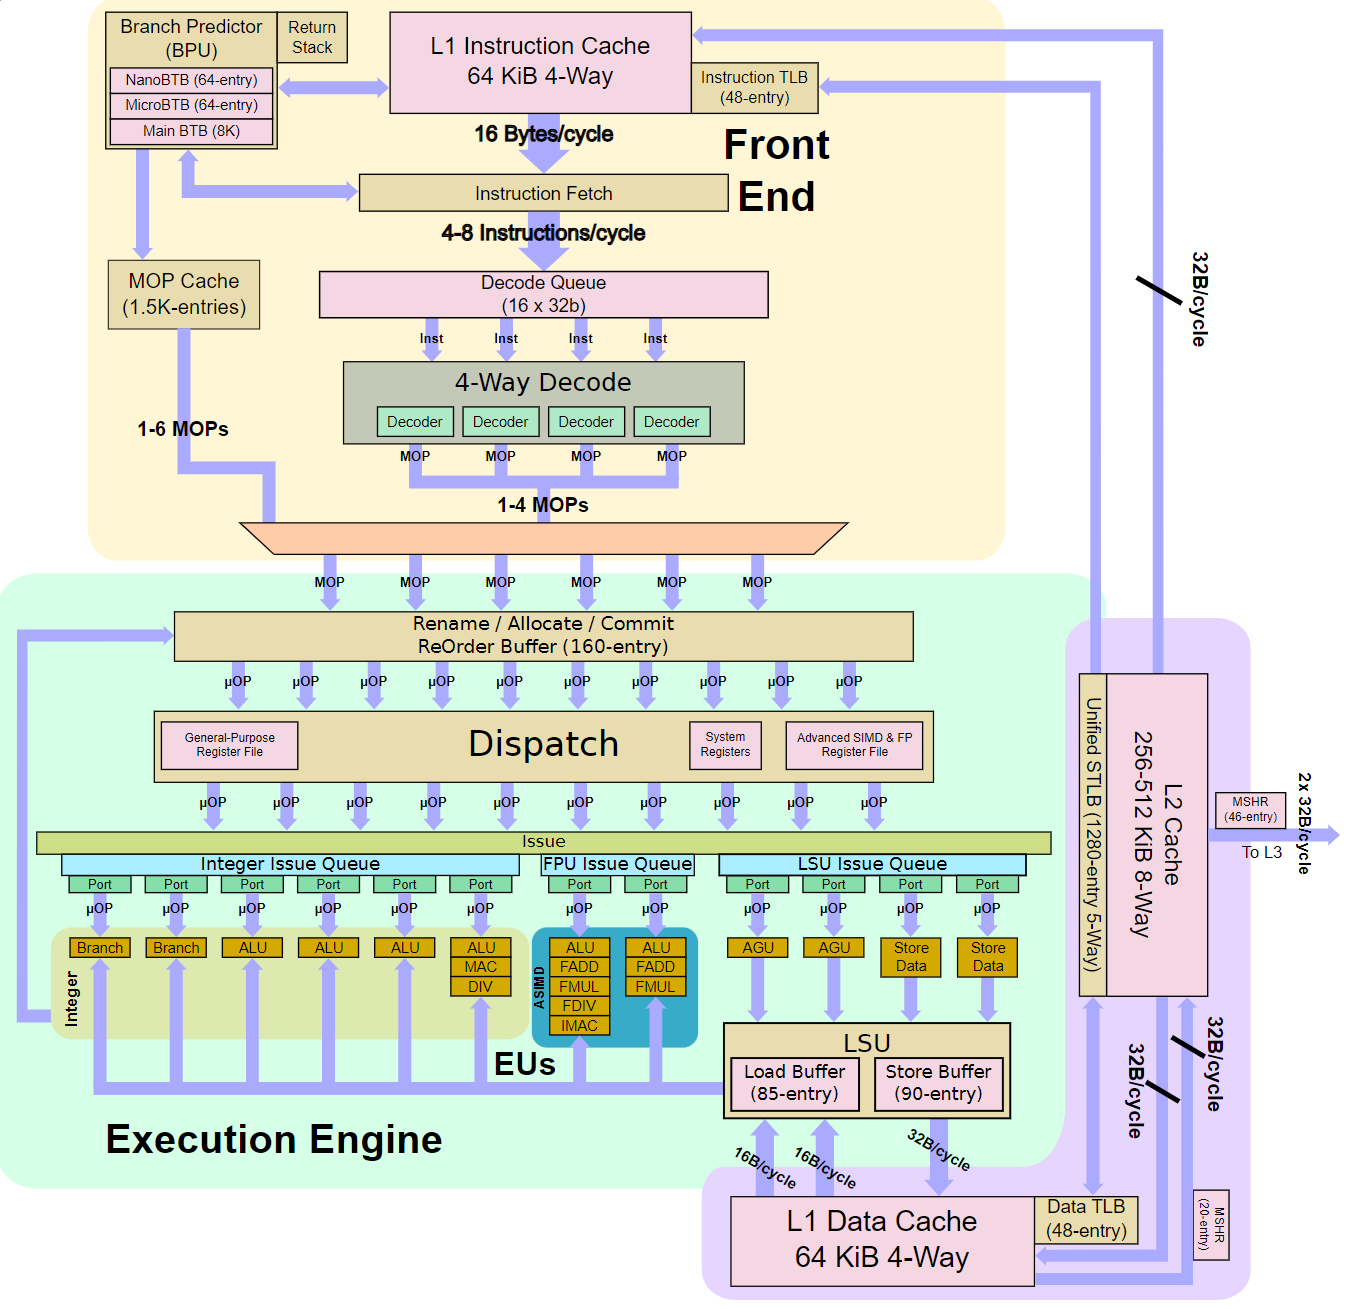
\includegraphics[width=161mm]{CortexA77}
        \label{cortexA77}
    \end{figure}

\subsubsection{Организация памяти}

    Процессор в современных мобильных системах встроен в так называемую SoC (System-on-chip --
    система на кристалле) систему -- электронная схема, которая выполняет цели компьютера
    и размещена на одной интегральной схеме. Таким образом, в такую систему встроены сразу процессор,
    таймеры, счётчики, интерфейсы для периферийных устройств, ОЗУ, ПЗУ и даже графический ускоритель.
    Именно таким образом устроены современные
    смартфоны, фотоаппараты, умные часы, элекронные книги и схожие устройства.

    Одна из основных подсистем системы на кристалле -- подсистема памяти. Наиболее быстродействующими
    элементами памяти являются регистры процессора, они же имеют наименьшее количество памяти, более
    высокую цену для производства и самую малую плотность расположения в электронной схеме.

    Учитывая малый объём возможного хранения данных с помощью регистров, а также
    что любая вычислительная система обладает локальностью (как по данным, так и по
    времени), почти всегда вводят дополнительные уровни памяти -- более дешёвые в производстве,
    имеющий больший объём и более высокую плотность ячеек хранения данных на электронной схеме.
    Более низкие уровни памяти являются кешами для более высоких.
    Таким образом, любая система имеет ОЗУ и кеши в качестве промежуточного хранилища данных
    (см. рис. \ref{CachePyramid}).

    Во всех современных мобильных системах в качестве ОЗУ используется LPDDR SDRAM
    (Low-Power Double Data Rate Synchronous Dynamic Random-Access Memory --
    динамическая оперативная память синхронного доступа с двойной скоростью передачи данных и
    с низким энергопотреблением). В дальнейшем для удобства будем использовать более простое
    обозначение для такой памяти -- DDR (Double Data Rate) память.

    Количество уровней кешей и объём их памяти напрямую зависят от требований к исполнению
    современных приложений и особенностей архитектуры мобильной системы,
    всегда являются компромиссом: с одной стороны, добавление дополнительного
    уровня кеша -- снижение вероятности обращения в DDR память (наиболее медленная память),
    а с другой -- введение постоянной дополнительной задержки при обращении в DDR, если данные
    в кешах отсутствуют.

    \begin{figure}[!h]
        \caption{Пример иерархии памяти в системе с 3-мя уровнями кешей}
        \centering
        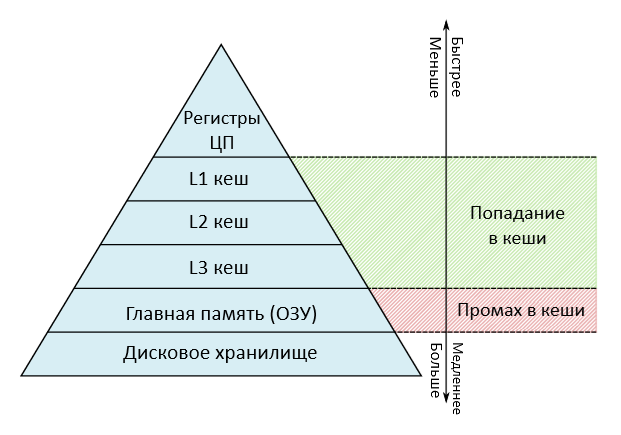
\includegraphics[width=116mm]{CachePyramidRU}
        \label{CachePyramid}
    \end{figure}

    Чаще всего производят мобильные устройства с 2-мя и более уровнями кешей. В системах на кристалле,
    как правило, последним (дополнительным) уровнем является системный кеш, который обычно
    не вносят в список уровней кешей процессора, так как он используется не только самим процессором,
    но также и различными периферийными устройствами, такими как графический ускоритель, ускоритель
    нейронных сетей и т.д..

    \begin{figure}[!h]
        \caption{Пример иерархии кешей в многоядерном процессоре (отсутствуют кеш 3-его уровня
            и системный кеш)}
        \centering
        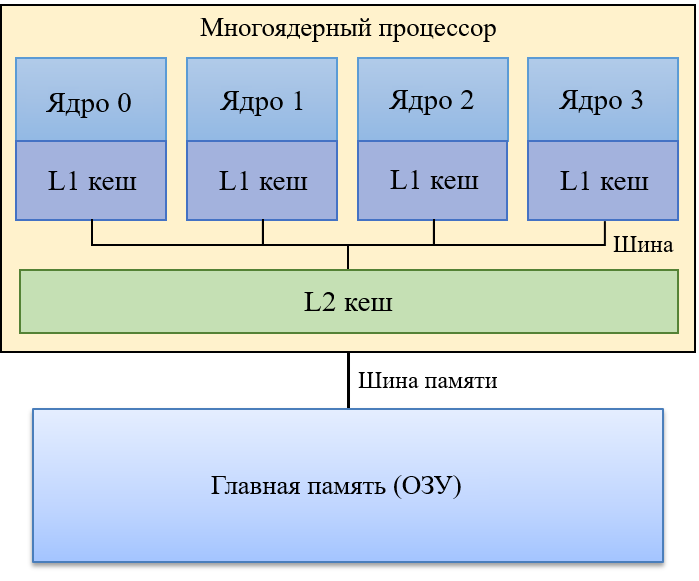
\includegraphics[width=95mm]{MulticoreCacheRU}
        \label{MulticoreCache}
    \end{figure}

    Каждое ядро процессора имеет кеш инструкций и кеш данных 1-ых уровней, на которые для краткости
    ссылаются как на единый кеш 1-ого уровня.
    При промахе в кеш 1-ого уровня поиск данных происходит в кеше 2-ого уровня, при промахе
    в кеш 2-ого -- поиск в кеше 3-его (если таковой имеется), и так до тех пор, пока не возникнет
    промах в системный кеш, после чего произойдёт обращение в DDR память
    (см. рис. \ref{MulticoreCache}).

    Как правило, кеш 2-ого уровня уникален для каждого ядра, хотя в некоторых гетерогенных системах
    кеш 2-ого уровня может использовать либо группой из 2-ух ядер в марках 1-ого кластера, либо
    целиком всем кластером ядер (такое поведение характерно для энергоэффективных ядер).
    Кеш 3-его уровня всегда разделяется между всеми ядрами системы, как и системный кеш вместе с ОЗУ.

    ПЗУ, а также компоненты для долгосрочного хранения данных (диски, твёрдотельные накопители и др.)
    в данной работе рассматриваться не будут.

\subsubsection{Технология DVFS} \label{dvfs_chapter}

    Почти все электронные схемы являются логическими элементами, которые имеют источник тактирования
    и работают на определённой частоте. Однако некоторым устройствам не выгодно работать при
    строго фиксированной частоте, например, если ядро процессора часто ждёт операции ввода-вывода,
    то эффективнее снизить рабочую частоту для более экономного расходования энергии, не сильно
    потеряв в производительности.

    Технология DVFS (Dynamic Voltage-Frequency Scaling) позволяет в режиме реального времени
    регулировать частоту и напряжение, с которыми работает устройство. Как правило, возможные значения
    частот являются дискретным набором, причём для каждой частоты существует минимальное значение
    напряжения, при котором устройство всё ещё остаётся в работоспособном состоянии.

    Практически все современные процессоры используют DVFS для регулировки частот ядер. В случае
    гетерогенных систем, т.е. имеющих кластеры ядер с различными характеристиками (например, более
    энергоэффективные или более производительные ядра),
    коими на сегодняшний день являются большинство мобильных систем,
    предоставляется возможным регулировать частоты только целиком всего кластера, то есть всех ядер,
    расположенных в нём, а не каждого ядра по отдельности.

    Регулирование частот и напряжений используется не только в случае процессорных ядер, но также
    и в других компонентах компьютерных систем: ОЗУ, шины, кеши и т.д..

    Наибольший интерес в данной работе представляет алгоритм регулирования частот процессорных ядер,
    регулирование частот прочих компонент рассматриваться не будет.

\subsection{Алгоритмы и эвристики регулирования частот процессора}

\subsubsection{Политики регулирования частот в ядре Linux}

    Самым распространнёным способом регулирования частот ядер процессора в ядре Linux является
    использование драйвера CPUfreq, который предоставляет несколько политик
    регулирования \cite{KernelCPUfreq}:
    \begin{enumerate}
        \item ''Performance'' -- частота ядра процессора выставляется в максимальное значение.
        \item ''Powersave'' -- частота ядра процессора выставляется в минимальное значение.
        \item ''Userspace'' -- частота ядра процессора выставляется пользователем.
        \item ''Ondemand'' -- частота ядра процессора выставляется в зависимости от утилизации ядра
            за последний промежуток времени.
        \item ''Conservative'' -- аналогично ''Ondemand'', но частота меняется менее резко, небольшими
            шагами.
        \item ''Schedutil'' \cite{KernelDocsSchedutil} -- аналогично ''Ondemand'', но утилизация отслеживается
            не для ядер процессора, а для каждого потока исполнения.
            Дополнительно используется более продвинутая система подсчёта
            утилизации потока исполнения: не только за последний промежуток времени и с учётом весов
            каждого промежутка времении (более давние промежутки менее важны). В случае использования
            не CFS (Completely Fair Scheduler), а дедлайн планировщика (DL) или реального времени (RT)
            частота выставляется в максимальное значение.
    \end{enumerate}

    Политика ''Performance'' приводит к излишнему энергопотреблению, ''Powersave'' -- к потере
    производительности. ''Ondemand'' и ''Conservative'' -- не отслеживают утилизацию отдельно по
    потокам исполнения, к тому же не учитывают, что утилизация может быть нелинейна относительно частоты
    (например, если процессор проводит основное время в ожидании выполнения транзакции-чтения из памяти),
    поэтому могут выставлять заведомо завышенное значение частоты, что приводит к дополнительному
    энергопотреблению.

    ''Schedutil'' устраняет большинство недостатков политик регулирования частот, рассмотренных выше,
    но всё же он не учитывает возможную нелинейность утилизации от частоты ядра процессора.

    Ещё один существенный недостаток всех политик, рассмотренных выше, является предположение,
    что частоты любого ядра процессора может изменяться независимо от остальных.
    Как было упомянуто в \ref{dvfs_chapter}, в современных мобильных системах ядра группируются
    в кластеры и частоты могут меняться только целиком для всего кластера.

\subsubsection{Подсчёт утилизации в планировщике ядра Linux}

    В ядре Linux на данный момент в стандартном планировщике CFS (Completely Fair Scheduler)
    используется решение \cite{KernelDocsCapacity}, в котором при подсчёте утилизации ядра
    процессора рабочей нагрузкой учитывается тот факт, что ядра различного типа
    (в разных кластерах) имеют разную производительность, и что в рамках одного ядра
    производительность меняется в зависимости от выбранной частоты.

    Однако авторы такого решения полностью пренебрегли тем фактом, что отношение максимальных
    производительностей двух различных ядер не является константой, а сильно зависит от
    исполняемой рабочей нагрузки. Также не учтено, что зависимость производительности, измеряемой
    в количестве исполненных инструкций в единицу времени, обычно нелинейна относительно частоты процессора
    (так как скорость исполнения инструкций упирается не только в частоту ядра, но и в характеристики
    памяти).

    Таким образом, авторы вводят величины ёмкости работы ядра процессора (максимально возможной утилизации),
    выражающей производительность ядра в виде максимально возможных значений выполненных инструкций в
    единицу времени, и утилизации ядра рабочей нагрузкой за фиксированный интервал времени $\tau$,
    которая инвариантна относительно выбора ядра процессора и частоты:

    \begin{equation}
        util = \frac{\Delta t}{\tau} \cdot \frac{freq_{cpu_{i}}}{freq^{max}_{cpu_{i}}} \cdot
               \frac{capacity_{cpu_{i}}}{capacity^{max}_{cpu_{i}}} =
            inv_{i, freq},
    \end{equation}
    где $\Delta t$ -- суммарное время работы $i$-ого ядра процессора за промежуток времении $\tau$ с
    частотой $freq_{cpu_{i}}$. $freq^{max}_{cpu_{i}}$ -- максимально возможная частота $i$-ого ядра
    процессора, $capacity_{cpu_{i}}$ -- ёмкость $i$-ого ядра, характеризующая его производительность,
    и $capacity^{max}_{cpu_{i}}$ -- максимальная ёмкость среди всех ядер системы.

    Ёмкости вычисляются единожды с помощью измерений в конкретных сценариях исполнения
    (рабочих нагрузках) и применяются во всех остальных случаях без каких-либо обоснований, причём
    с линейной зависимостью от частоты ядра, что тоже неверно (в большистве случаев), т.к.
    такая зависимость определяется рабочей нагрузкой.

    В реальности используется утилизация, подсчитанная сразу за несколько промежутков времени
    (обычно одинаковых по длительности), например, PELT (Per Entity Load Tracking)
    \cite{KernelDocsSchedutil} использует экспоненциально движующееся
    среднее значение утилизаций из подсчитанных по формулам выше за определённые промежутки времени.

    В качестве альтернативы PELT, который официально представлен в ядре Linux, компанией Google
    был разработан WALT (Window Assisted Load Tracking) \cite{QualcommWALT}, который предназначен
    специально для мобильных устройств, где важна быстрая реакция со стороны ядра на изменение
    нагрузки процессора, чтобы не потерять в производительности.
    WALT считает утилизацию за существенно меньшее количество промежутков времени (5 вместо 32) и без
    экспоненциально движущихся средних значений, но алгоритм подсчёта утилизации за 1 промежуток времени
    совпадает с описанным выше.

    При выборе политики регулирования частот в Linux ''Schedutil'' \cite{KernelDocsSchedutil},
    WALT или PELT используются не только внутри планировщика, но и для выбора частоты ядра процессора, т.е.
    ''Schedutil'' переиспользует подсчитанное значение утилизации потока исполнения для регулирования
    частот (только в случае CFS планировщика).

    Таким образом, в данное время ни стандартный планировщик, ни подсистемы регулирования частот
    ядра Linux не учитывают особенности влияния рабочих нагрузок на производительность
    ядер процессора.

\subsubsection{Альтернативные алгоритмы регулирования частот}

    [тут очередной обзор литературы и пример работ на схожую тематику]



\subsection{Латентность памяти и утилизация её пропускной способности} \label{lat_util_chapter}

    Для построения модели производительности ядра процессора, т.е. для правильного подсчёта утилизации
    ядра и наиболее энергоэффективного регулирования частотами, важно учитывать не только структуру
    организации памяти в исследуемой системе, а также и динамические характеристики элементов
    такой системы. Наиболее важными характеристиками являются пропускная способность шин,
    соединяющих вычислительные подсистемы с подсистемами памяти, утилизация пропускной способности и
    латетность памяти -- промежуток времени между отправлением запроса на получение данных в память и
    между самим получением данных.

    Таким образом, кеши и DDR память имеют свои собственные динамические характеристики,
    приведённые ранее. Как правило, низкие уровни кешей работают на той же частоте, что
    и само процессорное ядро (группа ядер -- ядерный кластер), поэтому латентность таких кешей
    выражается через циклы ядра процессора, а не через абсолютное время. Сложнее ситуация обстоит
    с более высокими уровнями кешей и DDR памятью: они имеют отдельные источники тактирования,
    латентность выражается в аболютном времени, к тому же она зависит от утилизации
    пропускной способности шин, ведущих к этим элементам памяти, то есть от количества транзакций
    в единицу времени.

    В данной работе часть предлагаемой модели требует использования латентности памяти, поэтому
    необходимо рассмотреть существующие решения для её определения и/или возможного учёта в модели.

    Авторы работы \cite{keramidas2010interval} предлагают 2 модели для учёта латентности памяти
    в рамках алгоритма регулирования частот. Первая модель разбивает циклы процессора на 2
    компоненты: относящиеся к ожиданию транзакций памяти и
    относящиеся непосредственно к вычислительным блокам ядра процессора.
    Утверждается, что при изменении частоты ядра процессора изменяются только циклы, относящиеся к памяти
    (частота которой независима от частоты ядра).
    На этом и основывается алгоритм регулирования частот, использующий перерасчёт времени
    исполнения через циклы при различных частотах. Вторая модель является модификацией-улучшением
    первой модели: дополнительно предполагается, что в группе инструкций, которые обращаются в
    память подряд, следует учитывать только первую инструкцию в формуле для перерасчёта циклов,
    которые относятся к памяти, однако это требует наличие дополнительной информации на уровне кешей:
    среди всех промахов в кеши (т.е. обращений в следующий уровень памяти) следует учитывать только
    первые промахи среди группы промахов (промахов, находящихся на расстоянии порядка времени
    латентности обращения в вышележащие уровни памяти), что не поддерживается ни одним устройством.

    В работе также отмечается, что следует учитывать ROB в OoO процессорах: из циклов, относящихся к
    транзакциям памяти, следует вычесть ту часть циклов, которую тратит процессор на исполнение
    инструкций, расположенных в логическом порядке после инструкции-обращения в память,
    так как такие инструкции исполняются спекулятивно.

    В работе \cite{clapp2015quantifying} рассматривается подход использования аналитической
    формулы влияния утилизации пропускной способности памяти на её латентность, что влияет
    на производительность суперскалярного процессора в рамках рабочих нагрузок,
    связанных с областью вычислений больших данных.
    В этом подходе используется схожий принцип, предлагаемых в данной работе: использование как
    показателя производительности $cpi$ (отношения числа процессорных циклов к числу исполненных
    инструкций), которое включает в себя слагаемые, связанные с циклами, потраченными
    на время ожидания транзакций-обращений в память. Авторы вводят понятие блокирующего фактора
    для латентности: в зависимости от рабочей нагрузки при одинаковом количестве обращений в память
    влияние латентности на производительность ($cpi$) может меняться вплоть до десятка раз из-за
    параллельных обращений в память, что коррелирует с результатами работы \cite{keramidas2010interval}.
    При фиксированном блокирующем факторе значение $cpi$ зависит линейно от количества обращений
    в память в единицу инструкций.
    Таким образом, все рабочие нагрузки разделены на 2 вида: чувствительные к латентности (высокое
    значение блокирующего фактора) и чуствительные к пропускной способности (низкое значение
    блокирующего фактора).
    Однако данное исследование ограничивается
    рассмотрением обращений только в DDR память при фиксированных частотах всех устройств.

    Авторы работы \cite{eyerman2022dram} предлагает метод визуализации утилизации пропускной способности
    ОЗУ для выявления возможных мест оптимизации производительности: для этого они используют
    контроллер внутри ОЗУ для вычисления утилизации пропускной способности и латентности.

    Зависимость латентности от утилизации пропускной способности представляет собой монотонную
    возрастающую функцию, которую можно положить константой при значениях утилизации, не сильно близкой
    к максимально возможной (\cite{david2011memory}), при приближении утилизации к своему максимуму
    латентность начинает сильно расти.

    Таким образом, можно сделать основные выводы из существующих работ:
    \begin{enumerate}
        \item Чувствительность производительности к латентности памяти зависит от рабочей нагрузки и может
            быть очень низкой даже при большом количестве обращений в память (ОЗУ). Такая зависимость
            определяется уровнем параллелизма обращений в память.
        \item Латентность является монотонной возрастающей функцией от утилизации пропускной способности,
            которую можно приближённо положить константой почти на всём интеравале утилизации;
            при стремлении утилизации к своему пределу происходит быстрый рост латентности до значений,
            на порядки превышающих её нормальное значение.
    \end{enumerate}

\subsection{Симулятор архитектуры Gem5}

    При исследовании компьютерных архитектур, их оптимизации или оценки новых идей, связанных с
    параметрами таких архитектур, чаще всего используют не конечное устройство, а симуляцию
    архитектуры такого устройства, т.к. это и дешевле в разработке,
    и открывает больше возможностей в плане вариации параметров компонент архитектуры при оценке
    их влияния на разрабатываемое решение (оптимизация, алгоритм и т.д.).

    Одним из наиболее популярных и продвинутых симуляторов компьютерных систем является Gem5
    \cite{binkert2011gem5}. Он поддерживает различные архитектуры: ARM, ALPHA, MIPS,
    Power, SPARC, x86 и т.д.. Для симуляции возможно использовать несколько типов процессоров
    \cite{gem52017ArchExpl}, среди которых ''Atomic Simple'', ''Timing Simple'', ''Minor'',
    ''O3''. ''Atomic Simple'' является функциональной симуляцией машинных инструкций,
    ''Timing Simple'' -- простейшей потактовой модели исполнения машинных инструкций,
    ''Minor'' -- модель процессора, не поддерживающего спекулятивное исполнение (Out-of-Order),
    а ''O3'' -- поддерживающего спекулятивное исполнение.

    Gem5 поддерживает 2 режима симуляции: эмуляция системных вызовов (SE -- syscall emulation), который
    поддерживает симуляцию одного приложения с некоторыми ограничениями (например, ввиду отсутствия таблицы
    страниц, поддерживаемой операционной системой, обращения в виртуальную память упрощено, MMU (Memory
    Management Unit) не участвует в симуляции), и полная эмуляция системы (FS -- full system).

    В данной работе используется архитектура ARM, т.к. именно она используется в большинстве мобильных
    систем на сегодняшний день. В качестве процессора выбран процессор ''Minor'', т.к. он обеспечивает
    хорошую точность симуляции и на практике процессоры такого типа реально используются в мобильных
    устройствах в качестве энергоэффективных ядер. Процессор ''O3'' обладает более сложным конвейером и
    поддерживает внеочередное исполнение инструкций, такие ядра обычно используют как производительные
    (с повышенным энгергопотреблением), но симуляция такого типа процессорного ядра занимает больше
    времени, чем ''Minor'', поэтому он не выбран чисто из практических соображений.

    Компанией ARM в симуляторе Gem5 было разработано процессорное ядро HPI (High Performance In-order)
    \cite{gem52017HPI} на основе ''Minor'' специально для исследовательских целей. В дальнейшем
    будет использован именно этот тип процессорного ядра.

    В качестве режима симуляции выбрана полная эмуляция системы, которая поддерживает полноценный запуск
    ядра Linux под архитектуру ARM. Именно в режиме полной эмуляции будет произведено дальнейшее
    исследование-построение модели для регулирования частот процессорных ядер.

    %%About PMU counters (from arm site)
    %%About Gem5 PMU implementation

\newpage
